\documentclass{article}
\usepackage{amsmath}
\usepackage{mathtools}
\usepackage{gensymb}
\usepackage[a4paper,inner=1.5cm,outer=1.5cm,top=2cm,bottom=0.5cm]{geometry} 
\usepackage{xcolor}
\usepackage{tikz}
\usepackage{multicol}
\usepackage{pgfplots}
\usetikzlibrary{intersections}
\usetikzlibrary{intersections,calc,angles,quotes}
\usetikzlibrary{calc,angles,positioning,intersections,quotes,decorations.markings}
\usepackage{tkz-euclide}
\usetikzlibrary{backgrounds}
\usetikzlibrary{calc,through}
\usetikzlibrary{angles}
\usetikzlibrary{fadings}
\usetikzlibrary{shapes.geometric}
\usetikzlibrary{shapes.symbols}
\usepackage{draftwatermark}
\usepackage{mathptmx}

\SetWatermarkText{\textcolor{black!30}{Mathema Shukur}}
\SetWatermarkFontSize{2 cm}
\usepackage[utf8]{inputenc}
\usepackage{fontspec}

\setmainfont{[Kalpurush.ttf]}
\newfontface{\en}{[Arial.ttf]} %%this is optional, if you want to use a secondary font. Any english font is supported
\newlength\Radius
\setlength\Radius{4cm}
\begin{document} 
	\Large
	\textcolor{red}{Welcome To} 
	\\
	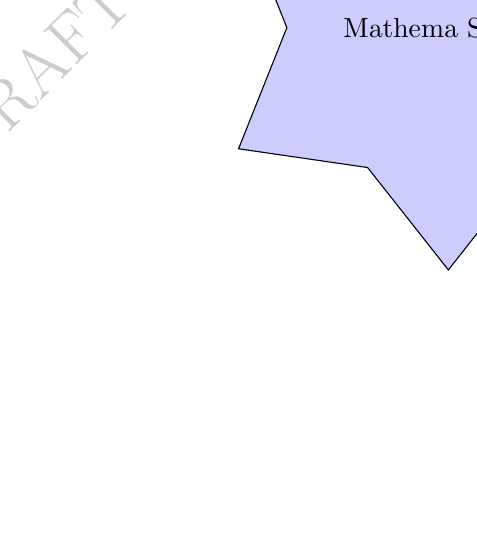
\begin{tikzpicture}
		\tikz \node [fill=blue!20,star,star points=6,draw] {Mathema Shukur };
	\end{tikzpicture}
\\
যাদের জন্যে প্রযোজ্যঃ  	\textcolor{magenta}{একাদশ ও দ্বাদশ শ্রেণীর শিক্ষার্থী} \\
বিষয়ঃ \textcolor{magenta}{উচ্চতর গণিত ১ম পত্র} \\
অধ্যায়ঃ \textcolor{magenta}{৩-সরলরেখা}\\ 
Subtopicঃ  \textcolor{magenta}{ কার্তেসীয় স্থানাঙ্ক ব্যবস্থার পরিচিতি }\\
\\ 
সতের শতাব্দীতে সর্ব প্রথম কার্তেসীয় স্থানাঙ্ক ব্যবস্থার (cartesian coordinate system) প্রচলন করেন ফরাসি গণিতবিদ ও দার্শনিক রেনে দেকার্তে ( Rene Descartes)।\\
\\
 কার্তেসীয় স্থানাঙ্ক ব্যবস্থা ইউক্লিডীয় জ্যামিতি (Euclidean geometry) এবং বীজগণিতের (algebra) মধ্যে সম্পর্কের ভিত্তি স্থাপন করে। এর ফলে এনালাইটিক্যাল জ্যামিতির (analytical geometry) যাত্রা শুরু হয়।\\
  এতে সরলরেখা, বক্ররেখা এবং বিভিন্ন জ্যামিতিক আকৃতি n মাত্রার ( n-dimensional) কার্তেসীয় সমতলে উপস্থাপন করা সহজ হয়।\\
\\
 কার্তেসীয় সমতলে লম্বভাবে পরস্পরছেদী দুইটি স্থির সরলরেখাকে অক্ষরেখা বিবেচনা করা হয়।\\
  ছেদ বিন্দুকে মূলবিন্দু $(0,0)$, আনুভূমিক রেখাকে $x$ অক্ষ এবং উলম্ব রেখাকে $y$  অক্ষ বিবেচনা করা হয়।\\
  $x$ অক্ষ ও  $y$ অক্ষ সমগ্র কার্তেসীয় সমতলকে চারটি ভাগে (quadrant) বিভক্ত করে ।\\
  \\
   আনুভূমিক দূরত্বকে ভুজ (Abscissa) এবং উলম্ব দুরত্বকে কোটি (Ordinate) বলা হয় । প্রথমে ভুজ পরে কোটি দ্বারা ক্রমজোড় (ordered pair) গঠিত হয়। এই ক্রমজোড় দ্বারা বিন্দুর স্থানাঙ্ক প্রকাশ করা হয় \\
 \\
 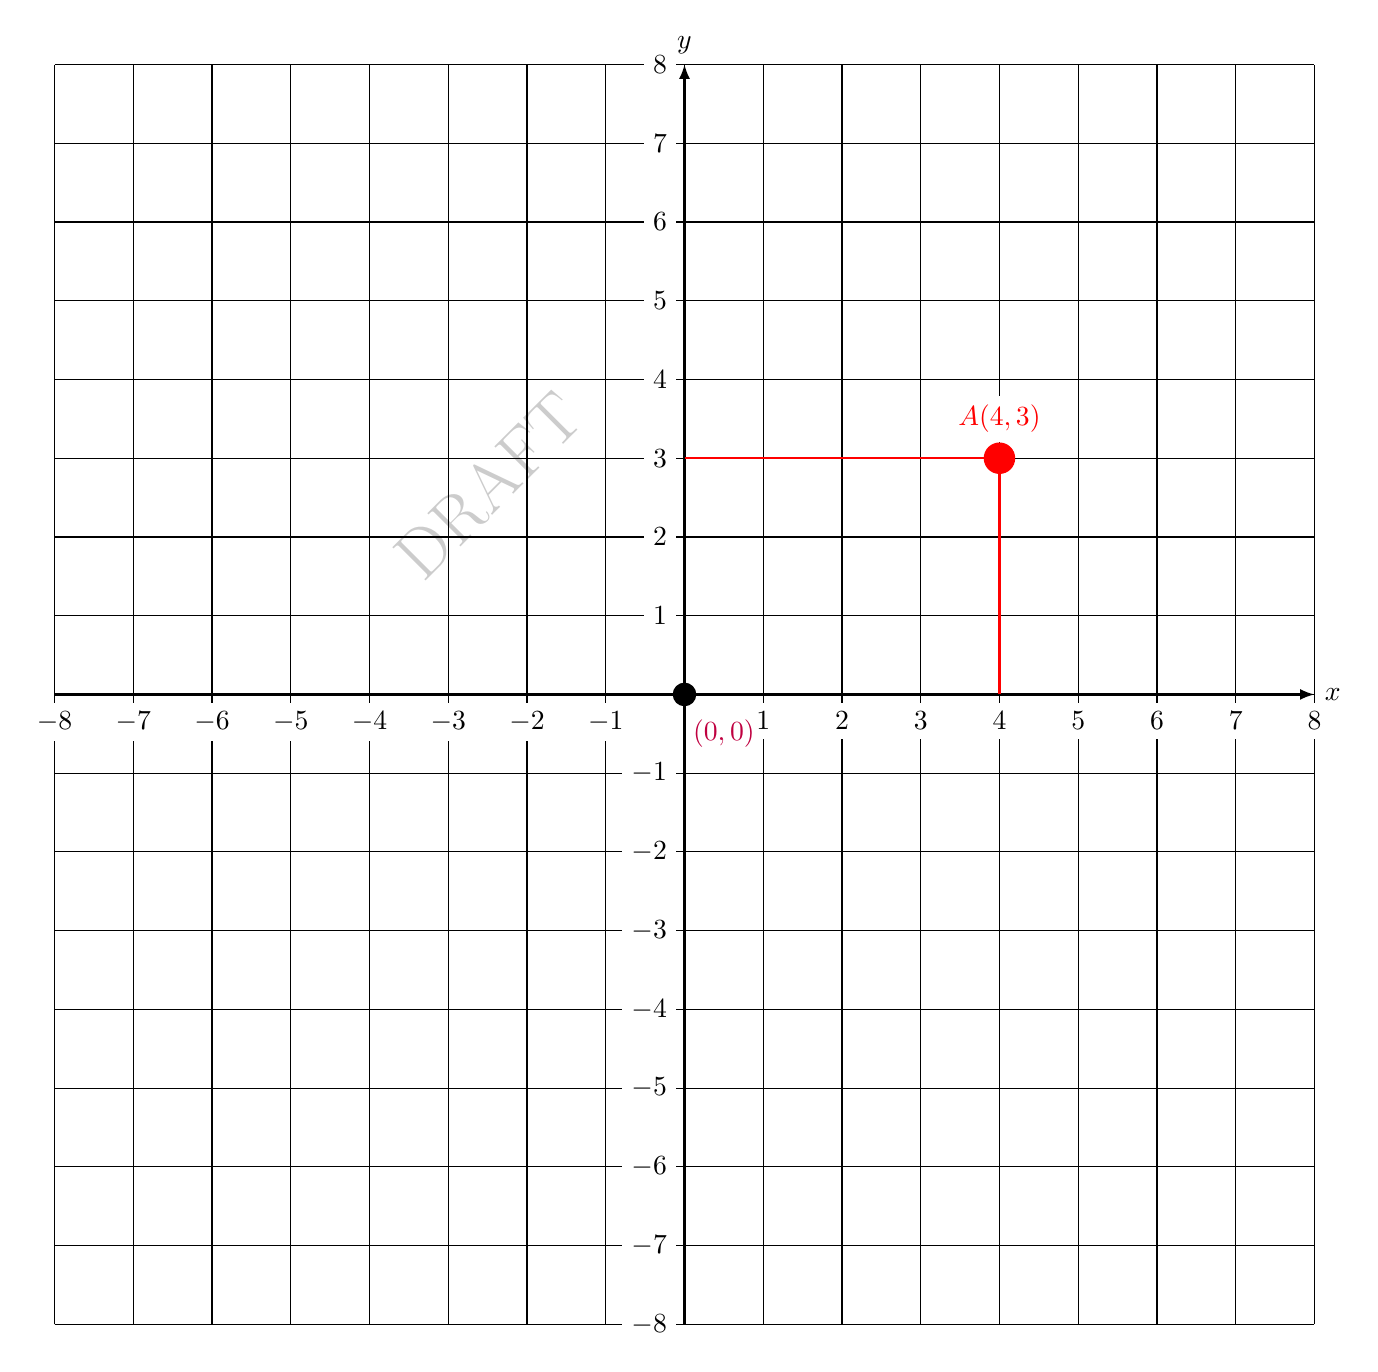
\begin{tikzpicture}[transform shape,scale=1]
 	\draw (-8,-8) grid (8,8);
 	\draw [-latex,thick](-8,0) -- (8,0) node[right] {$x$} coordinate(x axis);
 	\foreach \x in {-8,-7,-6,-5,-4,-3,-2,-1,1,2,3,4,5,6,7,8}
 	\draw (\x,0.1) -- (\x,-0.1) node [fill=white,below] {$\x$};
 	\draw [-latex,thick](0,-8) -- (0,8) node[above] {$y$} coordinate(y axis);
 	\foreach \y in {-8,-7,-6,-5,-4,-3,-2,-1,1,2,3,4,5,6,7,8}
 	\draw (0.1,\y) -- (-0.1,\y) node [fill=white,left] {$\y$};
 	\fill[black] (0,0) circle (1.5 mm);
 	\fill[red] (4,3) circle (2 mm);
 	\node[fill=white,above] at (4,3.2) {$\textcolor{red}{A(4,3)}$};
 		\node at (0.5,-0.5) {$\textcolor{purple}{(0,0)}$};
 	\draw[thick,red] (4,0)--(4,3);
 	\draw[thick,red] (0,3)--(4,3);
 \end{tikzpicture}
\\
\\  
১ম চতুর্ভাগে (First quadrant) প্রতিটি বিন্দুর ভুজ ও কোটি ধনাত্মক \\
\\
২য় চতুর্ভাগে (Second quadrant) প্রতিটি বিন্দুর ভুজ ঋণাত্মক, কোটি ধনাত্মক \\
\\
৩য় চতুর্ভাগে (Third quadrant) প্রতিটি বিন্দুর ভুজ ও কোটি ঋণাত্মক \\
\\
৪র্থ চতুর্ভাগে (Fourth quadrant) প্রতিটি বিন্দুর ভুজ ধনাত্মক , কোটি ঋণাত্মক \\
\\
 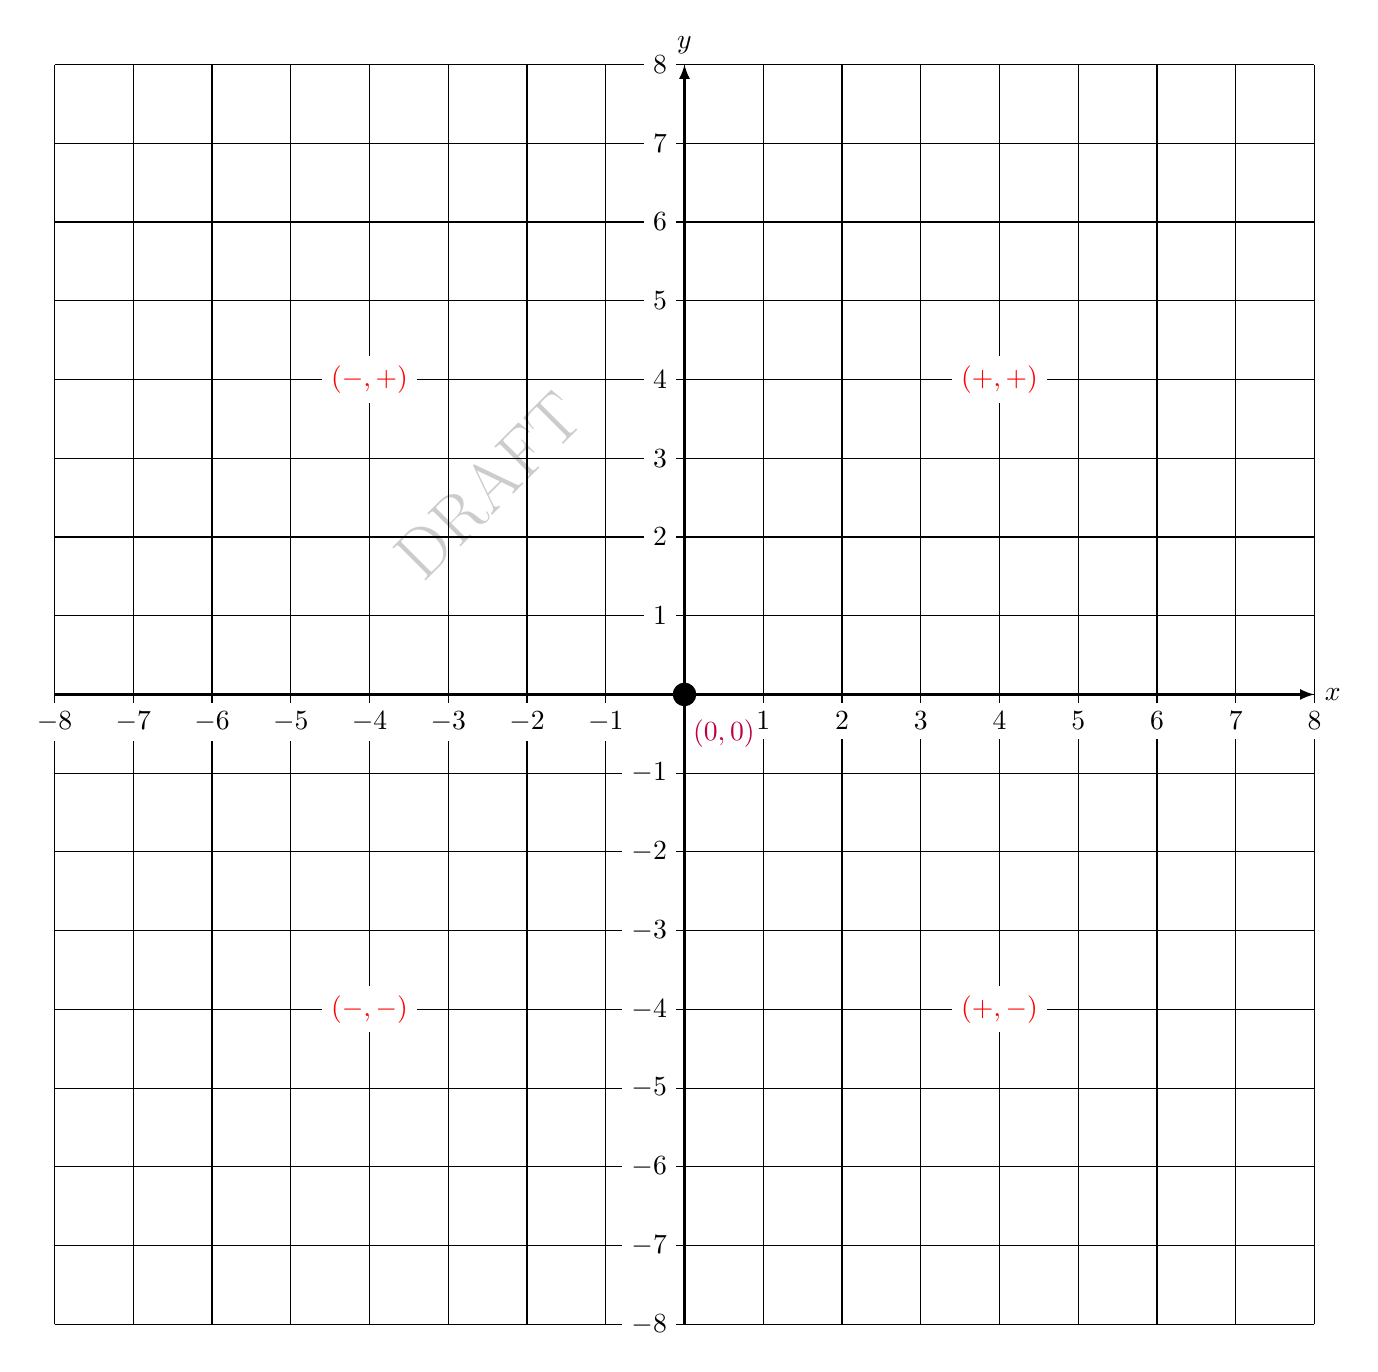
\begin{tikzpicture}[transform shape,scale=1]
	\draw (-8,-8) grid (8,8);
	\draw [-latex,thick](-8,0) -- (8,0) node[right] {$x$} coordinate(x axis);
	\foreach \x in {-8,-7,-6,-5,-4,-3,-2,-1,1,2,3,4,5,6,7,8}
	\draw (\x,0.1) -- (\x,-0.1) node [fill=white,below] {$\x$};
	\draw [-latex,thick](0,-8) -- (0,8) node[above] {$y$} coordinate(y axis);
	\foreach \y in {-8,-7,-6,-5,-4,-3,-2,-1,1,2,3,4,5,6,7,8}
	\draw (0.1,\y) -- (-0.1,\y) node [fill=white,left] {$\y$};
	\fill[black] (0,0) circle (1.5 mm);
		\node at (0.5,-0.5) {$\textcolor{purple}{(0,0)}$};
	\node[fill=white] at (4,4) {$\textcolor{red}{(+,+)}$};
		\node[fill=white] at (-4,4) {$\textcolor{red}{(-,+)}$};
			\node[fill=white] at (-4,-4) {$\textcolor{red}{(-,-)}$};
				\node[fill=white] at (4,-4) {$\textcolor{red}{(+,-)}$};
\end{tikzpicture}
\\
\\
$x$ অক্ষরেখার ওপর অবস্থিত প্রতিটি বিন্দুর কোটি শূন্য $(0)$। অর্থাৎ কোটি শূন্য হলে বিন্দুটি $x$  অক্ষের উপর অবস্থিত ।\\
\\
$y$  অক্ষরেখার ওপর অবস্থিত প্রতিটি বিন্দুর ভুজ শূন্য $(0)$ । অর্থাৎ ভুজ শূন্য হলে বিন্দুটি $y$ অক্ষের উপর অবস্থিত।\\
\\
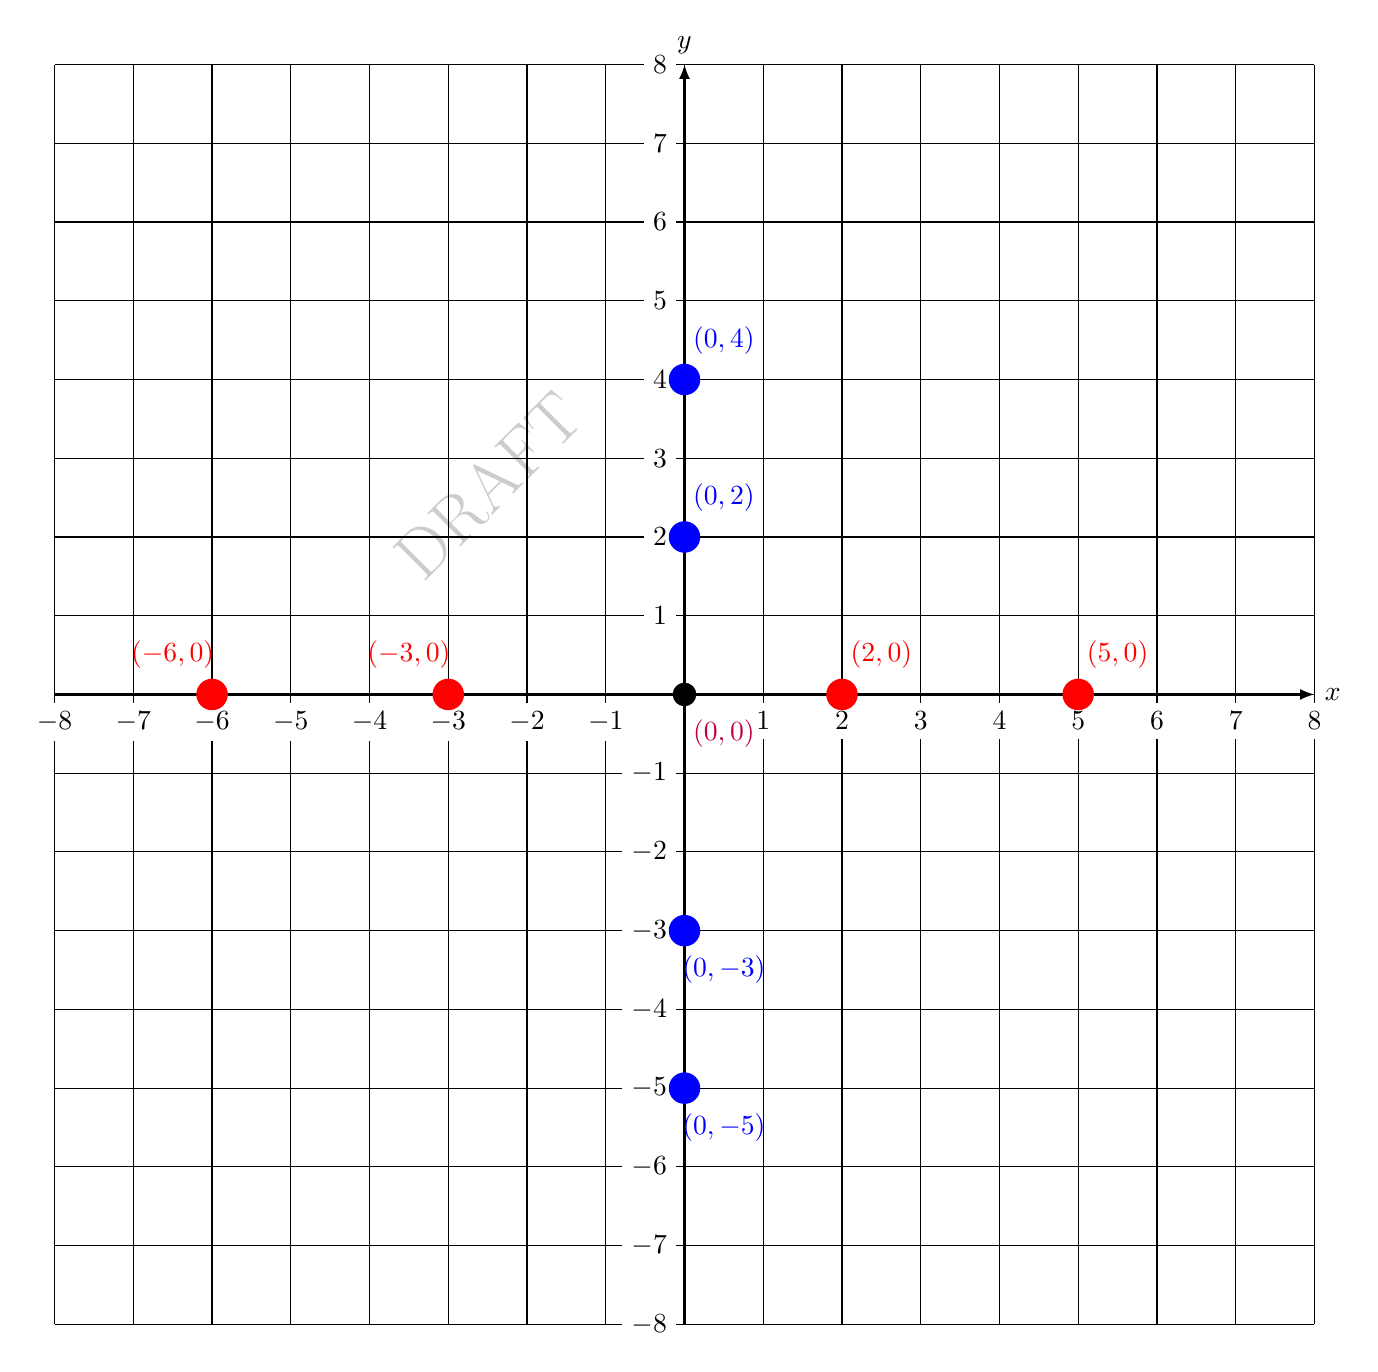
\begin{tikzpicture}[transform shape,scale=1]
	\draw (-8,-8) grid (8,8);
	\draw [-latex,thick](-8,0) -- (8,0) node[right] {$x$} coordinate(x axis);
	\foreach \x in {-8,-7,-6,-5,-4,-3,-2,-1,1,2,3,4,5,6,7,8}
	\draw (\x,0.1) -- (\x,-0.1) node [fill=white,below] {$\x$};
	\draw [-latex,thick](0,-8) -- (0,8) node[above] {$y$} coordinate(y axis);
	\foreach \y in {-8,-7,-6,-5,-4,-3,-2,-1,1,2,3,4,5,6,7,8}
	\draw (0.1,\y) -- (-0.1,\y) node [fill=white,left] {$\y$};
	\fill[black] (0,0) circle (1.5 mm);
		\node at (0.5,-0.5) {$\textcolor{purple}{(0,0)}$};
	\fill[red] (2,0) circle (2 mm);
		\fill[red] (5,0) circle (2 mm);
			\fill[red] (-3,0) circle (2 mm);
				\fill[red] (-6,0) circle (2 mm);
	\fill[blue] (0,2) circle (2 mm);
		\fill[blue] (0,4) circle (2 mm);
			\fill[blue] (0,-3) circle (2 mm);
				\fill[blue] (0,-5) circle (2 mm);
	\node at (2.5,0.5) {$\textcolor{red}{(2,0)}$};
	\node at (5.5,0.5) {$\textcolor{red}{(5,0)}$};
	\node at (-3.5,0.5) {$\textcolor{red}{(-3,0)}$};
	\node at (-6.5,0.5) {$\textcolor{red}{(-6,0)}$};
		\node at (0.5,2.5) {$\textcolor{blue}{(0,2)}$};
	\node at (0.5,4.5) {$\textcolor{blue}{(0,4)}$};
	\node at (0.5,-3.5) {$\textcolor{blue}{(0,-3)}$};
	\node at (0.5,-5.5) {$\textcolor{blue}{(0,-5)}$};
\end{tikzpicture}
\\
\vspace{5cm}
\\
$x$ অক্ষ হতে  $(x,y)$ বিন্দুর দূরত্ব  =|বিন্দুটির কোটি|=|y| একক \\
\\ 
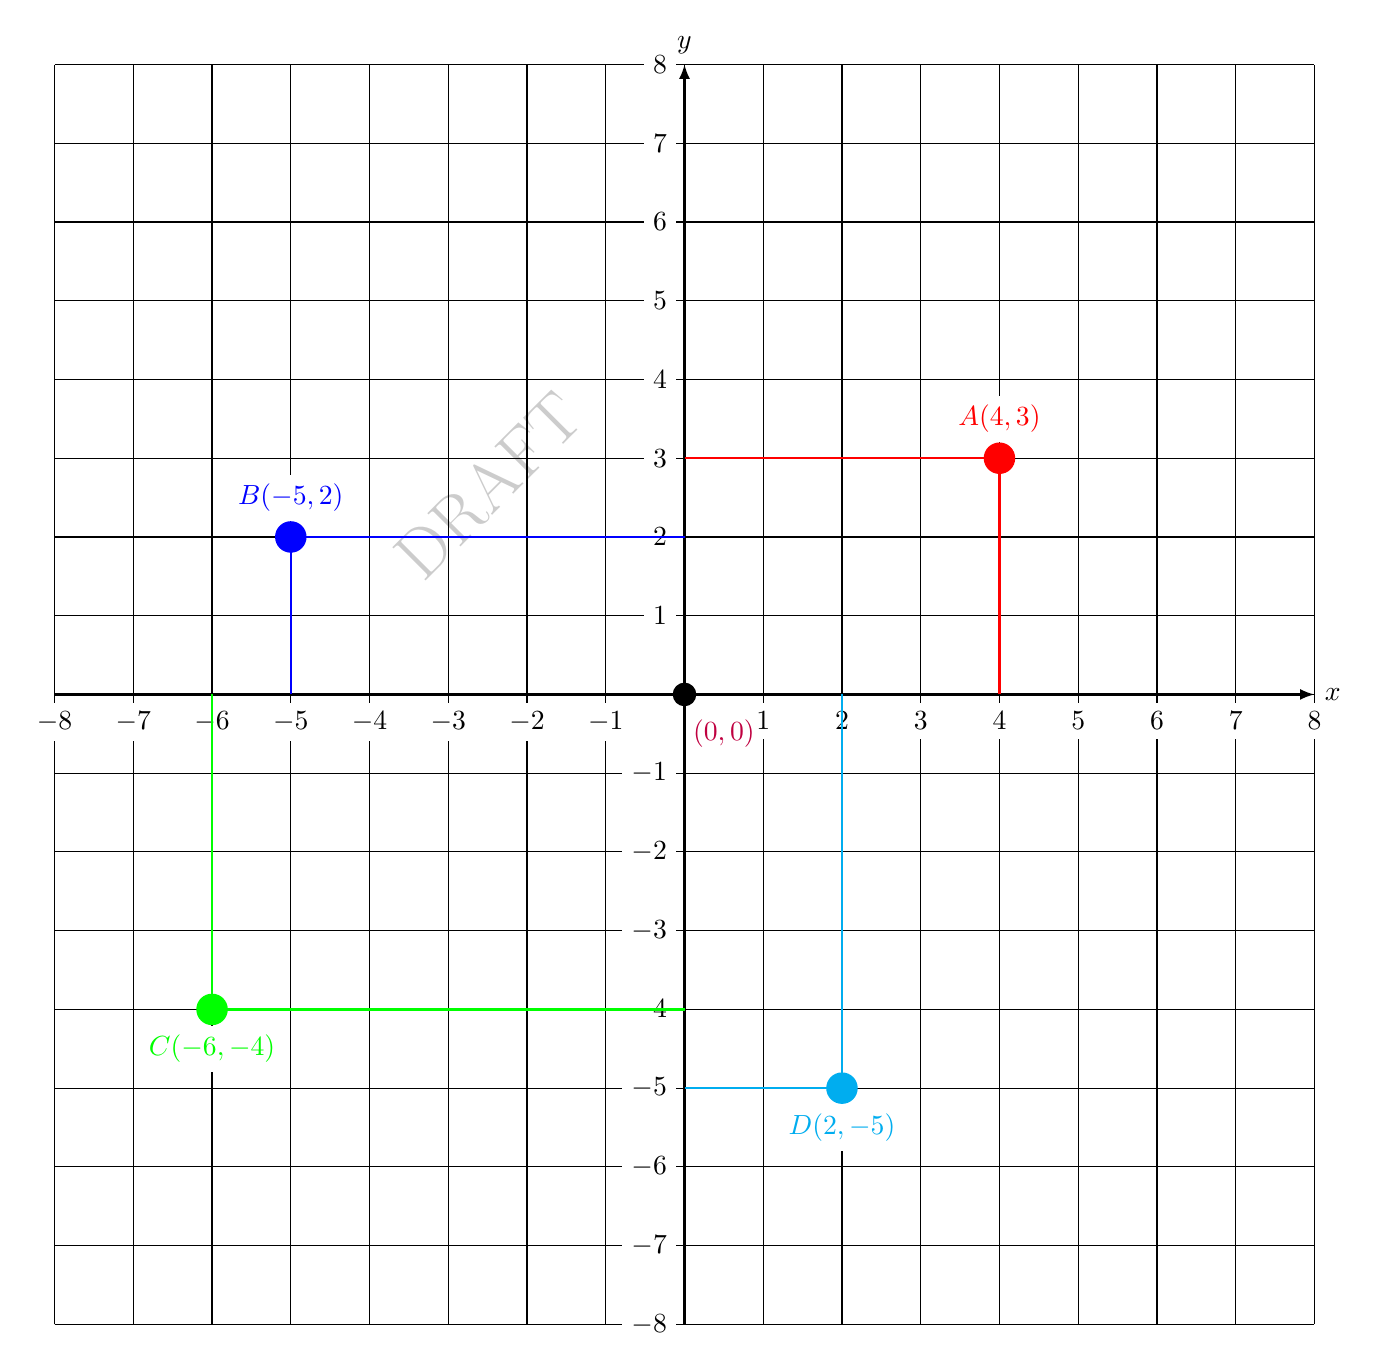
\begin{tikzpicture}[transform shape,scale=1]
	\draw (-8,-8) grid (8,8);
	\draw [-latex,thick](-8,0) -- (8,0) node[right] {$x$} coordinate(x axis);
	\foreach \x in {-8,-7,-6,-5,-4,-3,-2,-1,1,2,3,4,5,6,7,8}
	\draw (\x,0.1) -- (\x,-0.1) node [fill=white,below] {$\x$};
	\draw [-latex,thick](0,-8) -- (0,8) node[above] {$y$} coordinate(y axis);
	\foreach \y in {-8,-7,-6,-5,-4,-3,-2,-1,1,2,3,4,5,6,7,8}
	\draw (0.1,\y) -- (-0.1,\y) node [fill=white,left] {$\y$};
	\fill[black] (0,0) circle (1.5 mm);
		\node at (0.5,-0.5) {$\textcolor{purple}{(0,0)}$};
	\fill[red] (4,3) circle (2 mm);
	\fill[blue] (-5,2) circle (2 mm);
	\fill[green] (-6,-4) circle (2 mm);
	\fill[cyan] (2,-5) circle (2 mm);
	\node[fill=white,above] at (4,3.2) {$\textcolor{red}{A(4,3)}$};
	\node[fill=white,above] at (-5,2.2) {$\textcolor{blue}{B(-5,2)}$};
	\node[fill=white,below] at (-6,-4.2) {$\textcolor{green}{C(-6,-4)}$};
	\node[fill=white,below] at (2,-5.2) {$\textcolor{cyan}{D(2,-5)}$};
	\draw[thick,red] (4,0)--(4,3);
	\draw[thick,red] (0,3)--(4,3);
	\draw[thick,blue] (-5,0)--(-5,2);
	\draw[thick,blue] (0,2)--(-5,2);
	\draw[thick,green] (-6,0)--(-6,-4);
	\draw[thick,green] (0,-4)--(-6,-4);
	\draw[thick,cyan] (2,0)--(2,-5);
	\draw[thick,cyan] (0,-5)--(2,-5);
\end{tikzpicture}
\\
$x$ অক্ষ হতে  $B(-5,2)$ বিন্দুর দূরত্ব  =|2|=2একক \\
\\
$x$ অক্ষ হতে  $C(-6,-4)$ বিন্দুর দূরত্ব  =|-4|=4 একক \\
\\
\vspace{5cm}
\\
$y$ অক্ষ হতে  $(x,y)$ বিন্দুর দূরত্ব  =|বিন্দুটির ভুজ |=|x| একক \\
\\
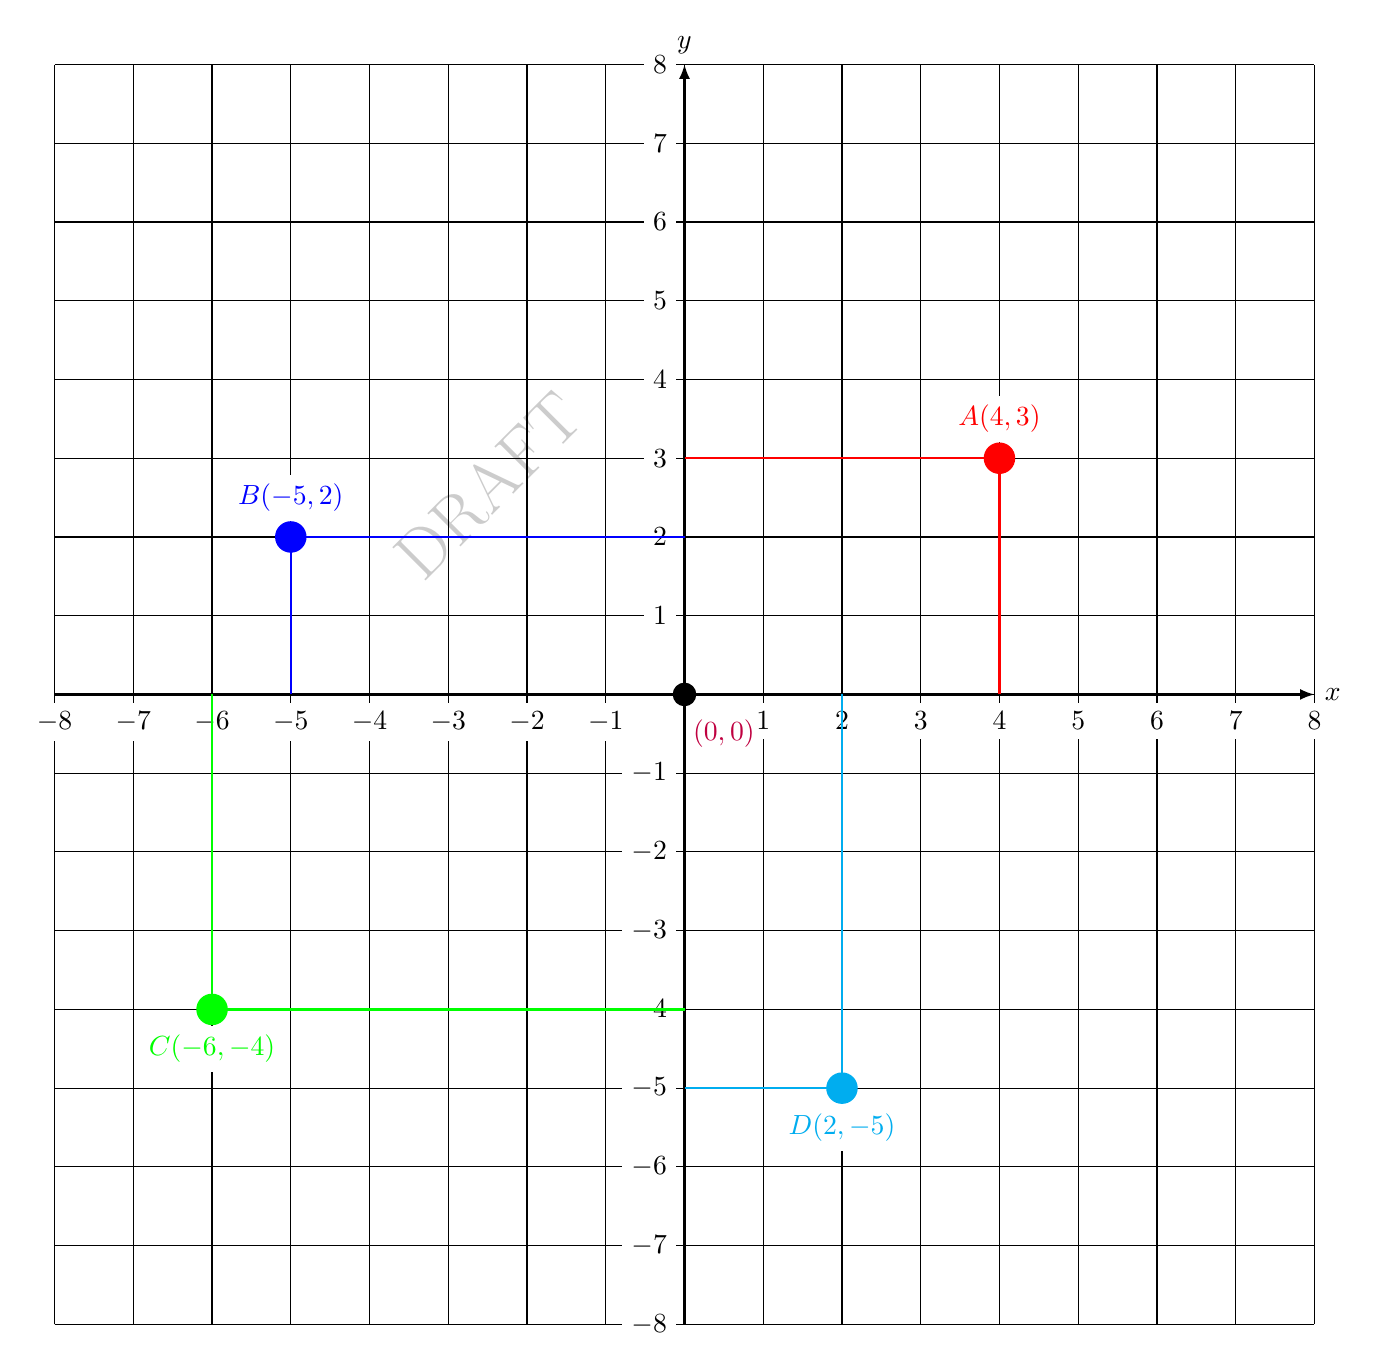
\begin{tikzpicture}[transform shape,scale=1]
	\draw (-8,-8) grid (8,8);
	\draw [-latex,thick](-8,0) -- (8,0) node[right] {$x$} coordinate(x axis);
	\foreach \x in {-8,-7,-6,-5,-4,-3,-2,-1,1,2,3,4,5,6,7,8}
	\draw (\x,0.1) -- (\x,-0.1) node [fill=white,below] {$\x$};
	\draw [-latex,thick](0,-8) -- (0,8) node[above] {$y$} coordinate(y axis);
	\foreach \y in {-8,-7,-6,-5,-4,-3,-2,-1,1,2,3,4,5,6,7,8}
	\draw (0.1,\y) -- (-0.1,\y) node [fill=white,left] {$\y$};
	\fill[black] (0,0) circle (1.5 mm);
		\node at (0.5,-0.5) {$\textcolor{purple}{(0,0)}$};
	\fill[red] (4,3) circle (2 mm);
	\fill[blue] (-5,2) circle (2 mm);
	\fill[green] (-6,-4) circle (2 mm);
	\fill[cyan] (2,-5) circle (2 mm);
	\node[fill=white,above] at (4,3.2) {$\textcolor{red}{A(4,3)}$};
	\node[fill=white,above] at (-5,2.2) {$\textcolor{blue}{B(-5,2)}$};
	\node[fill=white,below] at (-6,-4.2) {$\textcolor{green}{C(-6,-4)}$};
	\node[fill=white,below] at (2,-5.2) {$\textcolor{cyan}{D(2,-5)}$};
	\draw[thick,red] (4,0)--(4,3);
	\draw[thick,red] (0,3)--(4,3);
	\draw[thick,blue] (-5,0)--(-5,2);
	\draw[thick,blue] (0,2)--(-5,2);
	\draw[thick,green] (-6,0)--(-6,-4);
	\draw[thick,green] (0,-4)--(-6,-4);
	\draw[thick,cyan] (2,0)--(2,-5);
	\draw[thick,cyan] (0,-5)--(2,-5);
\end{tikzpicture}
\\
$y$ অক্ষ হতে  $D(2,-5)$ বিন্দুর দূরত্ব  =|2 |=2 একক \\
\\
$y$ অক্ষ হতে  $C(-6,-4)$ বিন্দুর দূরত্ব  =|-6 |=6 একক \\
\\
\vspace{5cm}
\\
মূলবিন্দু $(0,0)$ হতে যে কোনো বিন্দু $p(x,y)$ এর দূরত্ব  $d=\sqrt{x^2+y^2}$\\
\\
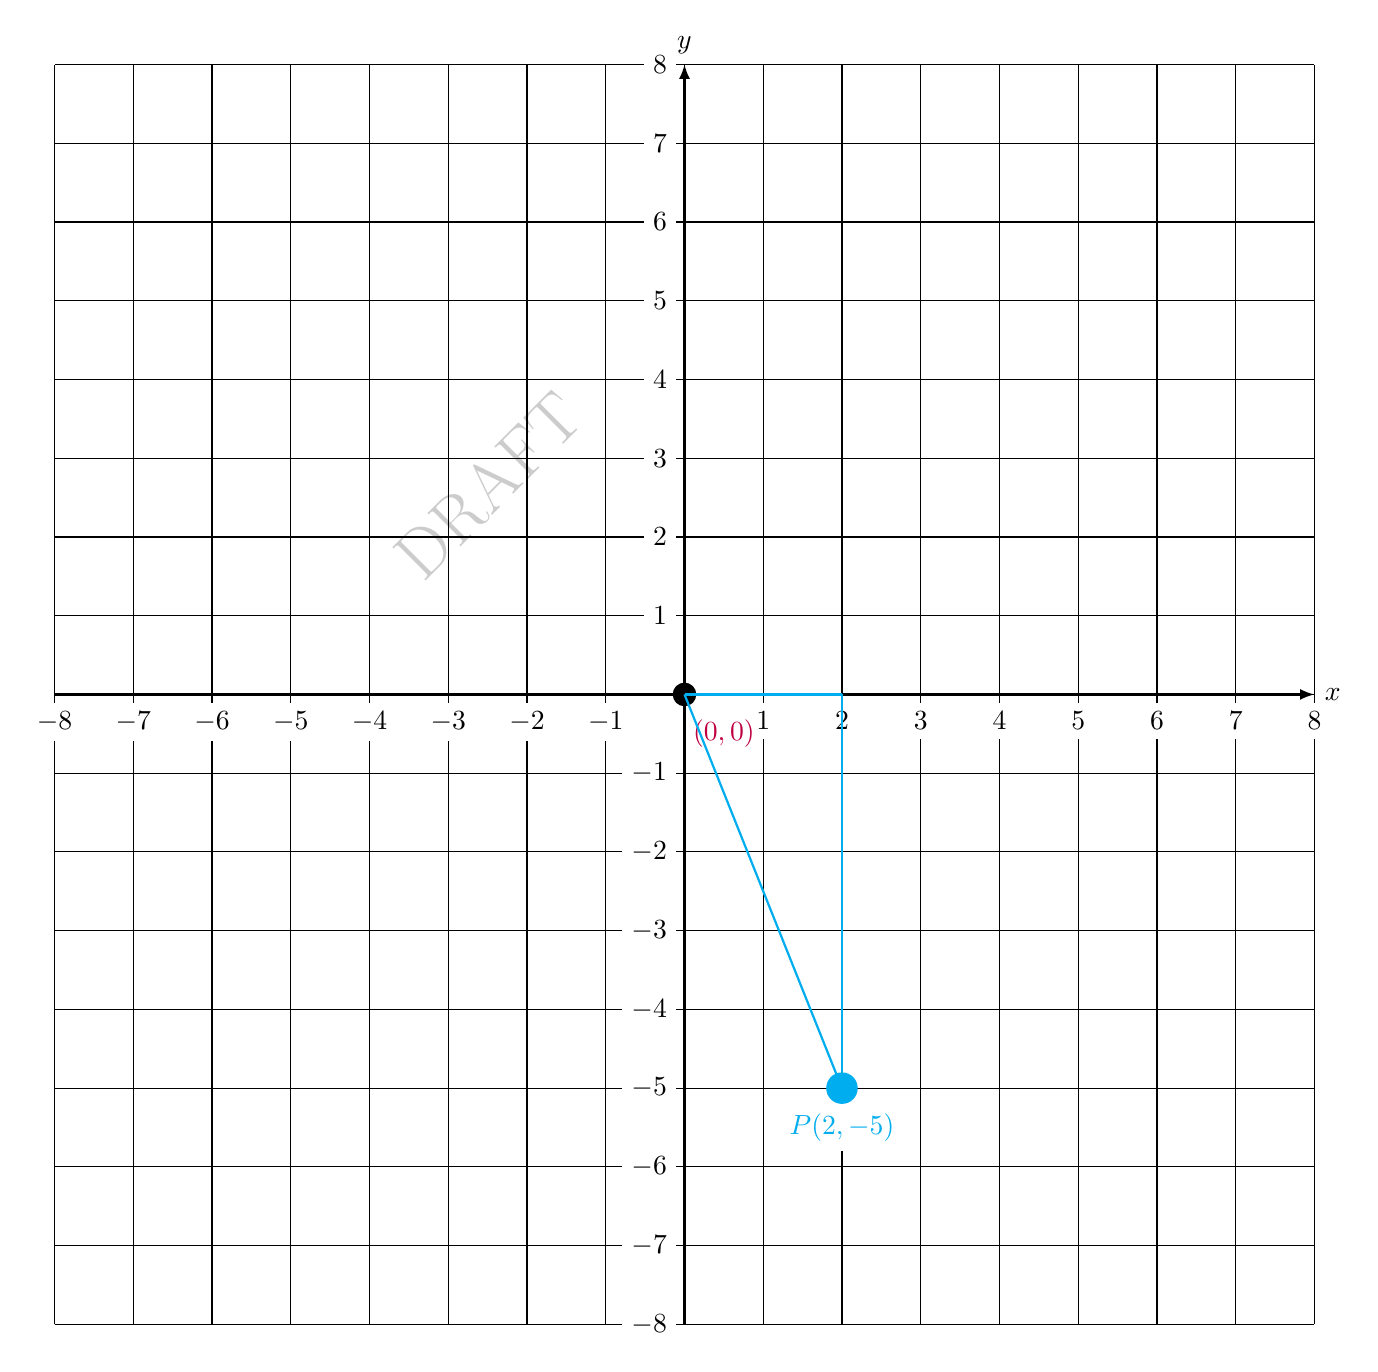
\begin{tikzpicture}[transform shape,scale=1]
	\draw (-8,-8) grid (8,8);
	\draw [-latex,thick](-8,0) -- (8,0) node[right] {$x$} coordinate(x axis);
	\foreach \x in {-8,-7,-6,-5,-4,-3,-2,-1,1,2,3,4,5,6,7,8}
	\draw (\x,0.1) -- (\x,-0.1) node [fill=white,below] {$\x$};
	\draw [-latex,thick](0,-8) -- (0,8) node[above] {$y$} coordinate(y axis);
	\foreach \y in {-8,-7,-6,-5,-4,-3,-2,-1,1,2,3,4,5,6,7,8}
	\draw (0.1,\y) -- (-0.1,\y) node [fill=white,left] {$\y$};
	\fill[black] (0,0) circle (1.5 mm);
	\node at (0.5,-0.5) {$\textcolor{purple}{(0,0)}$};
	\fill[cyan] (2,-5) circle (2 mm);
	\node[fill=white,below] at (2,-5.2) {$\textcolor{cyan}{P(2,-5)}$};
	\draw[thick,cyan] (2,0)--(2,-5);
	\draw[thick,cyan] (0,0)--(2,0);
	\draw[thick,cyan] (0,0)--(2,-5);
\end{tikzpicture}
\\
মূলবিন্দু $(0,0)$ হতে যে কোনো বিন্দু $P(2,-5)$ এর দূরত্ব  $d=\sqrt{(2)^2+(-5)^2}=\sqrt{29}$\\
\\
(ঢাকা বোর্ড-২০২১) $2x-3y+6=0$ রেখাটি  $x$ অক্ষকে যে বিন্দুতে ছেদ করে তার স্থানাঙ্ক নির্ণয় কর \\
\\
 $x$ অক্ষে যেকোনো বিন্দুর কোটি শূন্য অর্থাৎ $y=0$\\
 \\
 \begin{align*}
 	2x-3y+6&=0\\
 	\\
 		2x-3(0)+6&=0\\
 		\\
 		x&=-3
 \end{align*}
$2x-3y+6=0$ রেখাটি  $x$ অক্ষকে $(-3,0)$ বিন্দুতে ছেদ করে \\
\\
(দিনাজপুর  বোর্ড-২০২১) $3y-2x+6=0$ রেখাটি  $y$ অক্ষকে যে বিন্দুতে ছেদ করে তার স্থানাঙ্ক নির্ণয় কর \\
\\
$y$ অক্ষে যেকোনো বিন্দুর ভুজ শূন্য অর্থাৎ $x=0$\\
\\
\begin{align*}
3y-2x+6&=0\\
	\\
3y-2(0)+6&=0\\
	\\
	y&=-2
\end{align*}
$3y-2x+6=0$ রেখাটি  $y$ অক্ষকে $(0,-2)$ বিন্দুতে ছেদ করে \\
\end{document}